\documentclass{article}

% Language setting
% Replace `english' with e.g. `spanish' to change the document language
\usepackage[italian]{babel}

% Set page size and margins
% Replace `letterpaper' with`a4paper' for UK/EU standard size
\usepackage[letterpaper,top=2cm,bottom=2cm,left=3cm,right=3cm,marginparwidth=1.75cm]{geometry}

% Useful packages
\usepackage{listings}
\usepackage{xcolor}
\usepackage[utf8]{inputenc}
\usepackage[shortlabels]{enumitem}
\usepackage{amsmath}
\usepackage{graphicx}
\usepackage[export]{adjustbox} 
\usepackage[colorlinks=true, allcolors=blue]{hyperref}

\definecolor{codegreen}{rgb}{0,0.6,0}
\definecolor{codegray}{rgb}{0.5,0.5,0.5}
\definecolor{codepurple}{rgb}{0.58,0,0.82}
\definecolor{backcolour}{rgb}{0.95,0.95,0.92}

\lstdefinestyle{javastyle}{
    backgroundcolor=\color{backcolour},   
    commentstyle=\color{codegreen},
    keywordstyle=\color{magenta},
    numberstyle=\tiny\color{codegray},
    stringstyle=\color{codepurple},
    basicstyle=\ttfamily\footnotesize,
    breakatwhitespace=false,         
    breaklines=true,                 
    captionpos=b,                    
    keepspaces=true,                 
    numbers=left,                    
    numbersep=5pt,                  
    showspaces=false,                
    showstringspaces=false,
    showtabs=false,                  
    tabsize=2
}

\lstdefinestyle{bashstyle}{
    backgroundcolor=\color{backcolour},   
    commentstyle=\color{codegreen},
    keywordstyle=\color{magenta},
    numberstyle=\tiny\color{codegray},
    stringstyle=\color{codepurple},
    basicstyle=\ttfamily\footnotesize,
    breakatwhitespace=false,         
    breaklines=true,                 
    captionpos=b,                    
    keepspaces=true,                 
    showspaces=false,                
    showstringspaces=false,
    showtabs=false
}

\lstdefinestyle{bashstyle_table}{
    commentstyle=\color{codegreen},
    keywordstyle=\color{magenta},
    numberstyle=\tiny\color{codegray},
    stringstyle=\color{codepurple},
    basicstyle=\ttfamily\footnotesize,
    breakatwhitespace=false,         
    breaklines=true,                 
    captionpos=b,                    
    keepspaces=true,                 
    showspaces=false,                
    showstringspaces=false,
    showtabs=false
}

\title{Ingegneria del Software - NomeProgetto}
\author{
  Antonio Marini\\
  \texttt{559200}
  \and
  Riccardo Pacioni\\
  \texttt{551337}
  \and
  FirstName3, LastName3\\
  \texttt{123456}
  \and
  FirstName4, LastName4\\
  \texttt{123456}
}


\begin{document}
\maketitle

\newpage

\section{Casi d'uso e narrativa.}

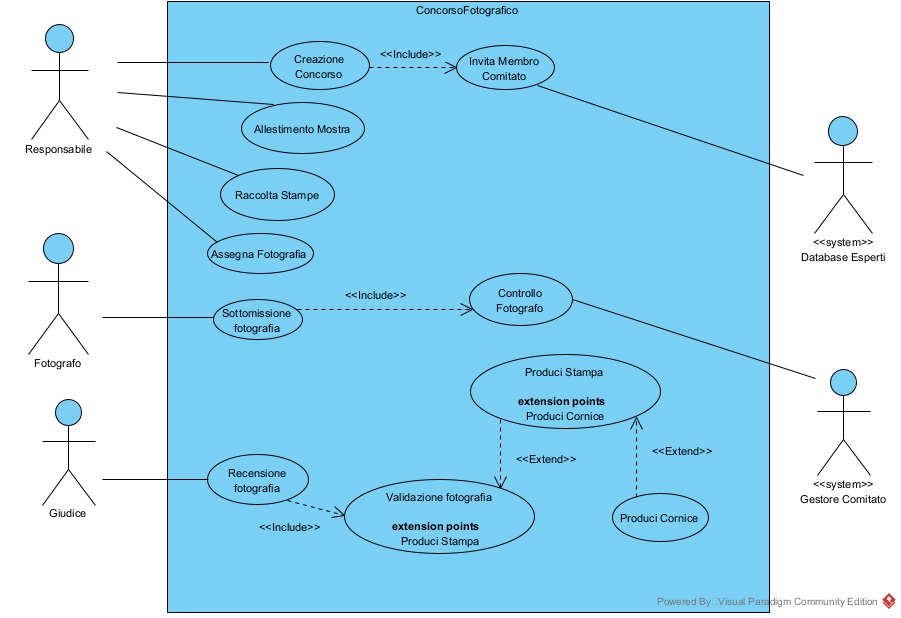
\includegraphics[max size={\textwidth}{\textheight}]{images/casiduso.png}

\begin{center}
    \begin{tabular}{ |r|p{9cm}| }
        \hline
        Nome                              & Creazione concorso                                                           \\
        \hline
        Descrizione                       & Azioni necessarie per creare un concorso fotografico e decidere il comitato. \\
        \hline
        Attori primari                    & Responsabile                                                                 \\
        \hline
        Attori secondari                  & Nessuno                                                                      \\
        \hline
        Precondizioni                     & Nessuna                                                                      \\
        \hline
        Sequenza principale degli eventi  &
        \begin{enumerate}
            \item Il responsabile richiede al sistema di creare un concorso
            \item Il sistema chiede i requisiti delle foto e numero massimo di foto
            \item Il sistema chiede la data e il luogo in cui tenere l’evento
            \item While(num giudici scelti $<$ $x$)
                  \begin{enumerate}
                      \item Mostra lista esperti disponibili ottenuta dal database degli esperti
                      \item Include Invita Membro Comitato
                  \end{enumerate}
        \end{enumerate}
        \\
        \hline
        Postcondizioni                    &
        \begin{itemize}
            \item Almeno un tema scelto,
            \item Requisiti fotografie scelti.
            \item Almeno $x$ giudici scelti.
            \item Concorso creato con successo.
        \end{itemize}
        \\
        \hline
        Sequenze alternative degli eventi &
        \begin{itemize}
            \item Ci sono meno di $x$ giudici nella base di dati
            \item Non ci sono date o luoghi disponibili per tenere l’evento
        \end{itemize}
        \\
        \hline
    \end{tabular}
\end{center}

\newpage

\section{Diagramma di sequenza.}
\section{Diagramma delle classi.}
\section{Diagramma macchina a stati.}
\section{Diagramma attività.}
\section{Architettura in vista C\&C e dislocazione.}
\section{Diagramma di struttura composita.}

\end{document}